% Scenario 1: Usability Enhancement through Standardized UIs
% Scenario: Efficient Data Retrieval for Tycoon Route Analysis and Account Information
\begin{table}[H]
    \centering
    \begin{tabularx}{\textwidth}{@{} lX @{}}
    \toprule
    \textbf{Aspect} & \textbf{Details} \\
    \midrule
    Source & Tycoon's analytical system requesting data for route pricing and passenger account details. \\
    Stimulus & The Tycoon system sends a data request to analyze route prices based on their subscription models and to gather specific account information for passengers. \\
    Artifact & Tycoon API interfacing between the Tycoon's systems and the TrIP system's databases. \\
    Response & The Tycoon API promptly routes the queries to the appropriate data providers, retrieves the requested information, and consolidates the results for the Tycoon system. \\
    Measure & Tycoon system receives comprehensive data within 3 seconds, enabling effective route and subscription analysis for passenger accounts. \\
    \bottomrule
    \end{tabularx}
    \caption{Scenario for Tycoon API Data Retrieval}
    \label{table:tycoon_api_data_retrieval}
\end{table}

% Scenario: Streamlined System Updates through MVC Pattern
\begin{table}[H]
    \centering
    \begin{tabularx}{\textwidth}{@{} lX @{}}
    \toprule
    \textbf{Aspect} & \textbf{Details} \\
    \midrule
    Source & TrIP system development team. \\
    Stimulus & The need to update the route pricing algorithm without affecting the user interface. \\
    Artifact & Model-View-Controller (MVC) pattern within the TrIP system. \\
    Response & Developers update the Pricing Model with the new algorithm, which automatically propagates changes to the relevant Views without requiring additional adjustments. \\
    Measure & The system update is deployed with zero downtime, and subsequent feature updates require 40\% less time due to decoupled architecture. \\
    \bottomrule
    \end{tabularx}
    \caption{Scenario for Maintainability - MVC Pattern}
    \label{table:mvc_maintainability}
\end{table}

% Scenario: Enhanced User Experience with MVC-Driven UI
\begin{table}[H]
    \centering
    \begin{tabularx}{\textwidth}{@{} lX @{}}
    \toprule
    \textbf{Aspect} & \textbf{Details} \\
    \midrule
    Source & Passenger using the TrIP system to manage travel. \\
    Stimulus & The passenger updates their travel preferences in the User Account View. \\
    Artifact & MVC pattern facilitating the User Account management. \\
    Response & The Controller processes the passenger's input, updates the User Account Model, and the View dynamically reflects the changes, providing immediate visual confirmation to the passenger. \\
    Measure & Passengers express a 90\% satisfaction rate with the ease of updating preferences, and the error rate in preference updates decreases by 50\%. \\
    \bottomrule
    \end{tabularx}
    \caption{Scenario for Usability - MVC-Driven UI}
    \label{table:mvc_usability}
\end{table}


\section{Development Viewpoint}
We start discussing the information viewpoint by analyzing stakeholder concerns that need to be addressed.
We individuated the following user stories:
\begin{itemize}
    \item User stories TODO
\end{itemize}

As a consequence, we decided to prioritize Quality Attributes for this view as indicated in Table~\ref{tab:development_view}.
\begin{table}[h!]
    \centering
    \resizebox{\textwidth}{!}{%
    \begin{tabular}{|l|c|c|c|c|c|c|c|c|c|}
      \hline
      & Usability & Performance & Security & Modifiability & Cost Efficiency & Availability & Safety & Integrability & Maintainability \\
      \hline
      Development View & 
      \cellcolor{gray!60}X & % Usability (2nd priority)
       & % Performance
       & % Security
       \cellcolor{gray!40}X& % Modifiability
       & % Cost Efficiency
       & % Availability
       & % Safety
       \cellcolor{gray!25}X& % Integrability
      \cellcolor{gray!90}X \\ % Maintainability (1st priority)
      \hline
    \end{tabular}
    }
    \caption{Development View Prioritized Quality Attributes}
    \label{tab:development_view}
\end{table}

\subsection{View: Broker pattern for Tycoon API}
\subsubsection{Model}
\begin{figure}[H]
    \centering
    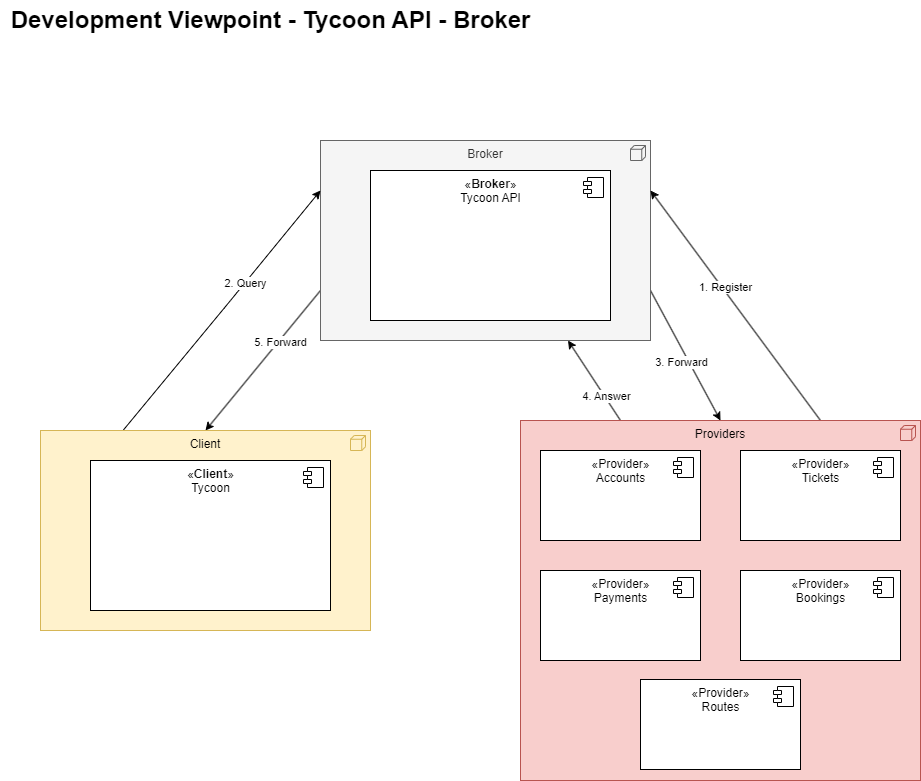
\includegraphics[width=\textwidth]{drawings/views_final_version/development_view_broker.png}
    \caption{Deployment view related broker pattern related to Tycoon API.}
    \label{fig:development_view_broker}
\end{figure}
\subsubsection{Description}
The diagram portrays the broker architecture in the TrIP system, delineating the communication between clients, the broker, and providers. Tycoon clients initiate the interaction by registering with the Tycoon API broker. Queries are sent from the Tycoon to the broker, which then forwards these queries to the relevant providers. These providers include services for Accounts, Payments, Bookings, Tickets, and Routes, each playing a pivotal role in processing Tycoon requests. Upon gathering the necessary data or performing the required actions, providers send their response back to the broker. The broker, in turn, forwards this information back to the Tycoon client, completing the request-response cycle. This broker pattern facilitates a structured approach to handling requests and centralizes the communication logic, simplifying interactions across the system’s diverse components.
\subsubsection{Glossary of Elements}

\begin{table}[H]
    \centering
    \caption{Glossary for the Broker in the Development View.}
    \label{tab:broker_development_glossary}
    \begin{tabular}{@{}llp{10cm}@{}}
        \toprule
    \textbf{Id} & \textbf{Name} & \textbf{Description} \\
    \midrule
    1 & Client & Represents the Tycoon requesting data or action from the broker. \\
    2 & Broker & Tycoon API that mediates between clients (Tycoon's) and various service providers (TrIP System's modules), handling requests and responses. \\
    3 & Provider & TrIP system that register with the broker to offer their services to clients. \\
    4 & Tycoon API & The application programming interface provided by the broker for communication with clients and providers. \\
    5 & Query & A request sent from the client to the broker, seeking information or action. \\
    6 & Register & The action of a provider adding their services to the broker's list of available resources. \\
    7 & Forward & The process of the broker sending requests to providers or responses back to clients. \\
    8 & Answer & The provider's response to a query that is sent back to the client via the broker. \\
    9 & Accounts & TrIP System module that manages user account information and authentication. \\
    10 & Tickets & TrIP system for issuing tickets, usually related to events or transportation. \\
    11 & Payments & The TrIP module that handles transaction processing. \\
    12 & Bookings & TrIP System module that manages reservations for services offered by the provider. \\
    13 & Routes & TrIP System module that handles route pricing. \\
    \bottomrule
    \end{tabular}
\end{table}
\subsubsection{Analysis on Perspectives}
\paragraph{Scenarios}
\scenarioOneDevelopment

\subsection{View: Model-View-Controller pattern for User Interface}
\subsubsection{Model}
\begin{figure}[H]
    \centering
    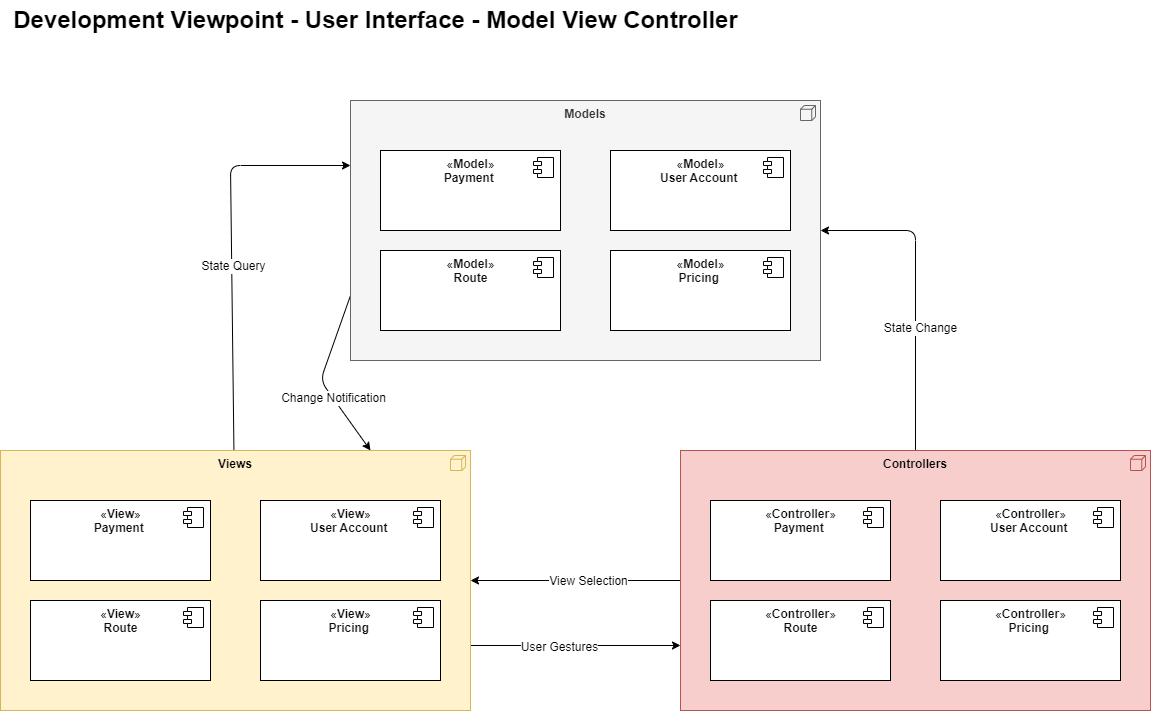
\includegraphics[width=\textwidth]{drawings/views_final_version/development_view_User_Interface.png}
    \caption{Development view model-view-controller pattern for UI}
    \label{fig:development_view_User_Interface}
\end{figure}

\subsubsection{Description}
This diagram illustrates the Model-View-Controller (MVC) pattern applied within the TrIP system. It breaks down the system's user interface into Views, which are responsible for presenting data to users and include interfaces for Payment, User Account, Route, and Pricing. The Models act as the data layer with Payment, Route, User Account, and Pricing components that manage the system's state. They receive state queries and broadcast state changes to the Views. Controllers interpret user gestures, direct state changes, and mediate between the Models and Views. This separation of concerns ensures that user interactions are handled efficiently, system data is managed cohesively, and business logic is executed in a controlled manner. The MVC architecture is fundamental to the system's organization, promoting clear delineations between different functionalities and facilitating ease of maintenance and scalability.

\subsubsection{Glossary of Elements}

\begin{table}[H]
    \centering
    \caption{Legend for the User Interface Components in the Development View of the TrIP System.}
    \label{tab:trip_system_ui_development_legend}
    \begin{tabular}{@{}llp{10cm}@{}}
    \toprule
    \textbf{Id} & \textbf{Name} & \textbf{Description} \\
    \midrule
    1 & Views & User interface components of the TrIP system that passengers interact with, including elements like payment, account management, and route selection screens. \\
    2 & Models & Data structures in the TrIP system that encapsulate the core business logic related to payment, user accounts, route information, and pricing. \\
    3 & Controllers & Components within the TrIP system that manage input from passengers, process requests, and produce responses by interacting with Models and updating Views. \\
    4 & Payment View/Model/Controller & Dedicated interfaces, data, and logic for processing passenger payments within the TrIP system, ensuring secure transactions. \\
    5 & User Account View/Model/Controller & Elements responsible for managing passenger profiles, including authentication and handling of personal account details in the TrIP system. \\
    6 & Route View/Model/Controller & Components that handle the presentation, data management, and operational logic of travel routes available to passengers in the TrIP system. \\
    7 & Pricing View/Model/Controller & The set of user interfaces, algorithms, and data that determine and manage fare calculations and display pricing information to passengers. \\
    8 & State Query & A request by the TrIP system to retrieve the current state, such as checking a passenger's account status or ticket validity. \\
    9 & State Change & An update within the TrIP system that alters the current state in response to passenger actions or other operational changes. \\
    10 & Change Notification & A notification mechanism that informs the TrIP system and passengers when a significant change has occurred, such as a payment confirmation or route update. \\
    11 & User Gestures & Interactions by passengers with the TrIP system, like touch or click actions, which are interpreted as commands to navigate or provide input. \\
    12 & View Selection & The process within the TrIP system for choosing the appropriate user interface view to display to passengers based on the current context or request. \\
    \bottomrule
    \end{tabular}
\end{table}

\subsubsection{Analysis on Perspectives}
\paragraph{Scenarios}
\scenarioTwoDevelopment
\scenarioThreeDevelopment

The Development Viewpoint focuses on the structural aspects that underpin the TrIP system's architecture, highlighting the modular approach in system design to enhance usability and maintainability. \\

\noindent \textbf{MVC Pattern:} \\
The adoption of the Model-View-Controller (MVC) pattern substantially improves the system's maintainability by segregating the user interface elements (Views) from the business logic (Models) and user input processing (Controllers). This separation of concerns allows developers to update or modify one aspect of the system — such as adding new features to the user interface — without the need to alter the underlying business logic or control flow. For passengers, this results in a more comprehensive interface with a variety of options and features, enhancing the overall usability of the system. The MVC pattern ensures that as passenger needs evolve, new Views can be added swiftly, making the system both adaptable and future-proof. \\

\noindent \textbf{Broker Architecture:} \\
In parallel, the broker architecture employed within the Tycoon API streamlines the interaction process between the Tycoons and the TrIP system. It serves as a centralized point for processing queries and handling communications, thus simplifying the complexity of these interactions. For the Tycoons, this architecture means usability is significantly enhanced, allowing them to communicate through a unified interface with the Tycoon API, which abstracts the intricate workings of the TrIP system's service modules. This consolidation of communication logic not only benefits the Tycoons but also reduces the overhead for the TrIP system in managing multiple communication protocols. \\

These architectural decisions, reflected in the Development Viewpoint, are key to the TrIP system's ability to offer an efficient, secure, and user-friendly platform that can grow and adapt in line with technological advancements and user expectations.
